\documentclass[11pt]{article}
\usepackage[top=1cm, bottom=2cm, left=1cm, right=1cm]{geometry}
\usepackage{ctex}
\usepackage{algorithm}
\usepackage{algorithmicx}
\usepackage{algpseudocode}
\usepackage{amsthm,amsmath,amssymb}
\usepackage[colorlinks=true,linkcolor=blue]{hyperref}
\usepackage{listings}
\usepackage{xcolor,xparse}
\usepackage{realboxes}
\usepackage{graphics}
\usepackage{graphicx}
\usepackage{mathrsfs}
\usepackage{wrapfig}
\usepackage{subfigure}
\usepackage{pifont}
\newcommand{\To}{\textbf{To} }
\definecolor{cmdbg}{rgb}{0.9,0.9,0.9}
\lstset{%
	basicstyle=\ttfamily,
	breaklines = true,
	backgroundcolor=\color{cmdbg},
}
\DeclareDocumentCommand{\ccmd}{v}{% 参数 v 表示工作方法类似于 \verb
    \Colorbox{cmdbg}{\csname lstinline\endcsname!#1!}%
}

\makeatletter
\newenvironment{breakablealgorithm}
  {% \begin{breakablealgorithm}
   \begin{center}
     \refstepcounter{algorithm}% New algorithm
     \hrule height.8pt depth0pt \kern2pt% \@fs@pre for \@fs@ruled
     \renewcommand{\caption}[2][\relax]{% Make a new \caption
       {\raggedright\textbf{\ALG@name~\thealgorithm} ##2\par}%
       \ifx\relax##1\relax % #1 is \relax
         \addcontentsline{loa}{algorithm}{\protect\numberline{\thealgorithm}##2}%
       \else % #1 is not \relax
         \addcontentsline{loa}{algorithm}{\protect\numberline{\thealgorithm}##1}%
       \fi
       \kern2pt\hrule\kern2pt
     }
  }{% \end{breakablealgorithm}
     \kern2pt\hrule\relax% \@fs@post for \@fs@ruled
   \end{center}
  }
\makeatother

\author{谢昀城 22307110070}
\title{计算物理作业2}

\begin{document}
\maketitle


\section{题目1:求方程的根}
\subsection{题目描述}
Sketch the function$x^3-5x+3=0$
\begin{enumerate}
    \item Determine the two positive roots to 4 decimal places using the bisection method. Note: You first need to bracket each of the roots.
    \item Take the two roots that you found in the previous question (accurate to 4 decimal places) and “polish them up” to 14 decimal places using the Newton-Raphson method.
    \item Determine the two positive roots to 14 decimal places using the hybrid method.
\end{enumerate}
\begin{figure}[!ht]
    \centering
    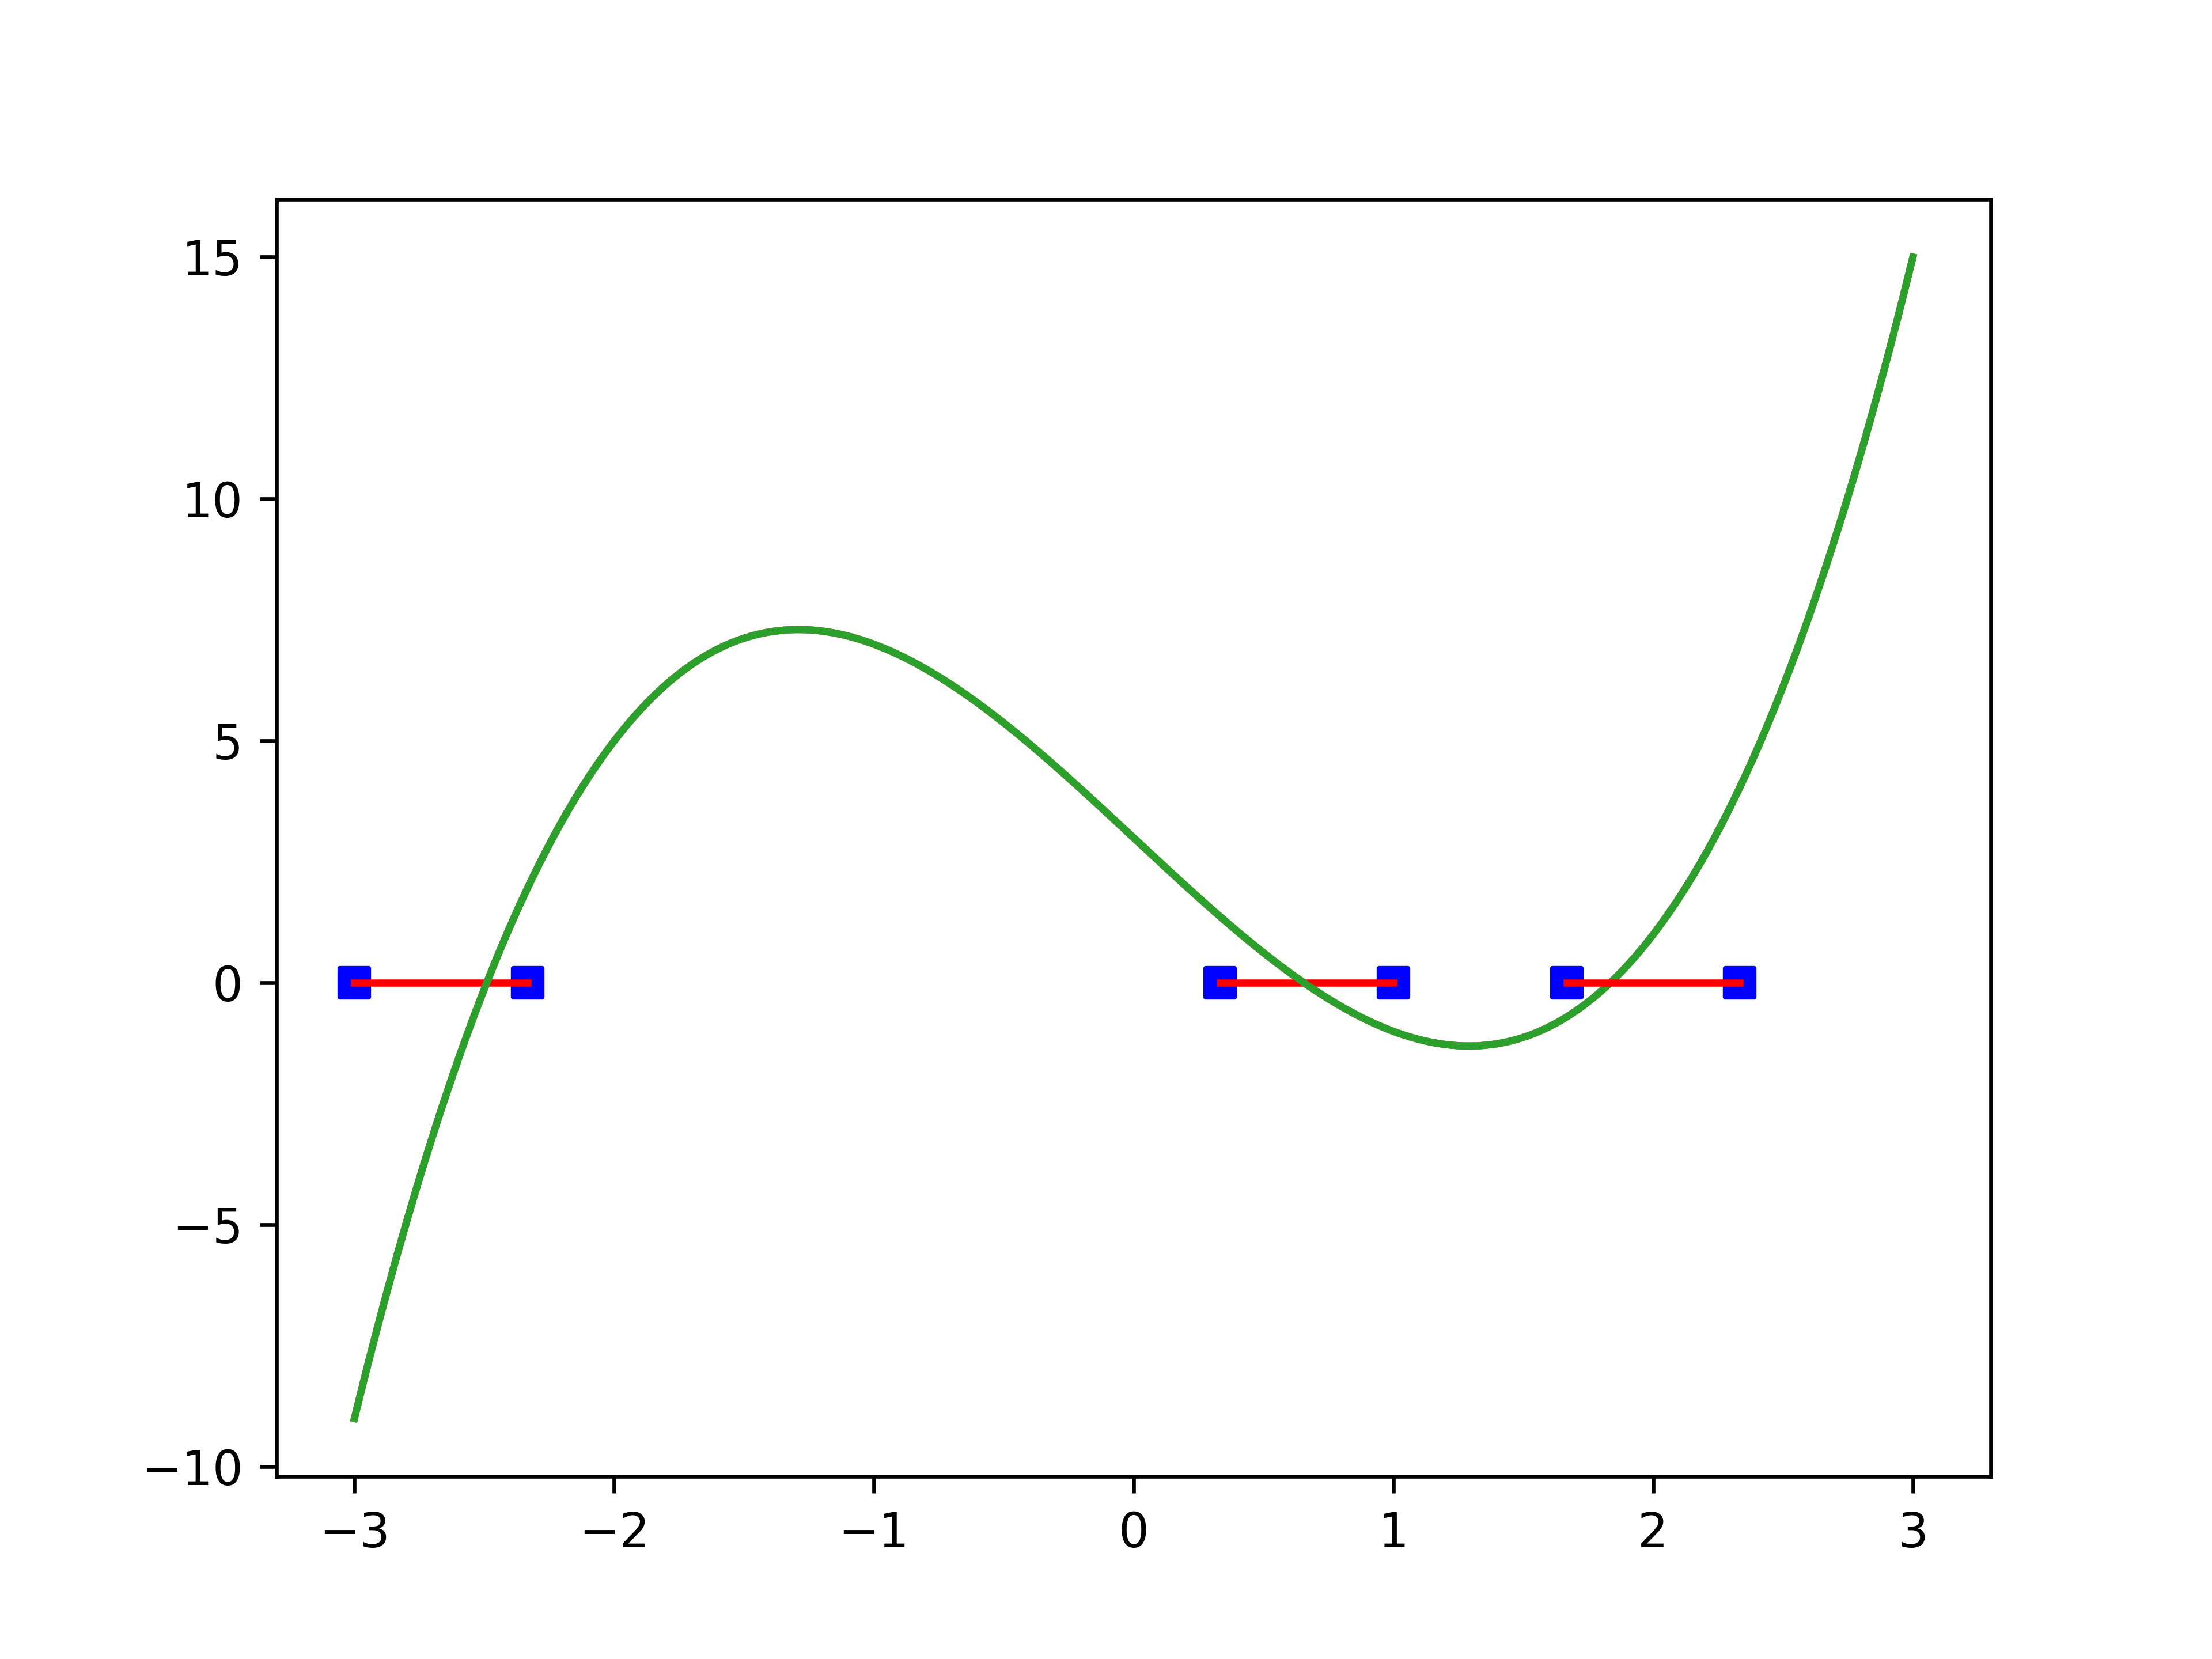
\includegraphics[width=0.6\linewidth]{photo/f(x) with bracket.png}
    \caption{f(x)-x图像。其中标出了由$find\_bracket$函数找出的变号区域}
    \label{fig:1}
\end{figure}

\subsection{程序描述}
对于题目要求求解的方程,我们首先通过在一定范围内均匀采样(一般采样10个点)找到其变号区间,在程序中由$find\_bracket$完成(见图\ref{fig:1})。对于1.1题,我们使用$bisection\_method$函数接收其变号区间,并在区间内使用二分法逼近其中的根,直到误差在容差$10^(-4)$以下,这里根的误差使用二分区间大小$|a-b|$估计。对于1.2和1.3题,由于np.float64类型浮点数的精度大约只有16位有效位数左右,因此我们使用decimal库实现50位有效数字的计算。我们在$newton_raphson_method$和$hybrid_method$函数中接收由1.1中得到的解,将其误差缩小至$10^(-14)$以下,这里误差我们使用$|f(x)/f'(x)|$估计。

本程序源文件为findroot.py,在终端进入当前目录,使用命令
\Colorbox{cmdbg}{\lstinline[language=bash]|python -u findroot.py|}
运行本程序。运行时请保证Python第三方库Numpy,Matplotlib,decimal已安装。程序开发环境为Python3.12.3,可在Python3.8以上版本中运行。

\subsection{伪代码}
\subsubsection{bisection method 伪代码:}
\begin{breakablealgorithm}
    \caption{FindBracket}
    \begin{algorithmic}
      \Function{FindBracket}{$f, rg, n, ifplot$}
        \State \textbf{INPUT:} $f$ (function), $rg$ (range), $n$ (number of points), $ifplot$ (boolean)
        \State \textbf{OUTPUT:} $bracket$ (list of tuples)
    
        \State $x \gets$ linspace($rg[0], rg[1], n$)
        \State $y \gets f(x)$
        \State $yRoll \gets roll(y, 1)$
        \State $yCov \gets y[1:] * yRoll[1:]$
        \State $cr0 \gets where(yCov < 0)$ \Comment{Convolve 2 series to find the cross point}
        \State $bracket \gets [(x[i], x[i+1]) \text{ for } i \text{ in } cr0[0]]$
        \State \Return $bracket$
      \EndFunction
    \end{algorithmic}
    
\end{breakablealgorithm}

\subsubsection{bisection method 伪代码:}
\begin{breakablealgorithm}
  \caption{BisectionMethod}
  \begin{algorithmic}
    \Function{BisectionMethod}{$f, rg, tol, maxIter$}
      \State \textbf{INPUT:} $f$ (function), $rg$ (range), $tol$ (tolerance), $maxIter$ (maximum iterations)
      \State \textbf{OUTPUT:} $(root, error)$ (root of the function and the error)
  
      \State $a, b \gets rg$
      \If{$f(a) * f(b) \geq 0$}
        \State \textbf{Raise} ValueError("Function does not change sign in the interval.")
      \EndIf
      \For{$i \gets 0$ \To $maxIter - 1$}
        \State $c \gets (a + b) / 2$
        \If{$|b - a| < tol$} \Comment{Convergence condition, using $|a - b|$ as the error}
          \State  \textbf{print the root and Break}
        \ElsIf{$f(c) * f(a) < 0$}
          \State $b \gets c$
        \Else
          \State $a \gets c$
        \EndIf
      
      \EndFor
      \State \Return $(a + b) / 2, |b - a|$
    \EndFunction
  \end{algorithmic}
  \end{breakablealgorithm}
  
\subsubsection{Newton-Raphson method 伪代码:}
\begin{breakablealgorithm}
  \caption{NewtonRaphsonMethod}
  \begin{algorithmic}
    \Function{NewtonRaphsonMethod}{$fDecimal$, $dfDecimal$, $x0$, $tol$, $maxIter$}
      \State \textbf{INPUT:} $fDecimal$ (function), $dfDecimal$ (function), $x0$ (initial point), $tol$ (tolerance), $maxIter$ (maximum iteration)
      \State \textbf{OUTPUT:} $x$ (root), $error$ (absolute error)
      
      \State $x \gets$ Decimal($x0$) \Comment{Convert $x0$ to decimal type}
      \State $tol \gets$ Decimal($tol$) \Comment{Convert $tol$ to decimal type}
  
      \For{$i \gets 1$ \To $maxIter$}
        \State $fx \gets fDecimal(x)$
        \State $dfx \gets dfDecimal(x)$
        
        \If{$dfx = 0$}
          \State \textbf{Raise} ValueError("Meet zero derivative at", $x$)
        \EndIf
        
        \State $dx \gets fx / dfx$
        
        \If{$|dx| < tol$}
          \State\textbf{print the root and Break}
        \EndIf
        
        \State $x \gets x - dx$
      \EndFor
      
      \State \Return $x$, $|dx|$
    \EndFunction
  \end{algorithmic}
  \end{breakablealgorithm}

\subsubsection{Hybrid method 伪代码:}
  \begin{breakablealgorithm}
    \caption{HybridMethod}
    \begin{algorithmic}
      \Function{HybridMethod}{$f$, $df$, $rg$, $tol$, $maxIter$}
        \State \textbf{INPUT:} $f$ (function), $df$ (derivative of $f$), $rg$ (range), $tol$ (tolerance), $maxIter$ (maximum iteration)
        \State \textbf{OUTPUT:} $x$ (root), $error$ (absolute error)
        
        \State $a,b \gets$ Decimal($rg$) \Comment{Convert range to decimal type}

        \State $eps \gets 10^{5 - \text{environment precision}}$
        \State $x \gets (a + b) / 2$
        
        \If{$f(a) * f(b) \geq 0$}
          \State \textbf{Raise} ValueError("Function does not change sign in the interval.")
        \EndIf
        
        \For{$i \gets 1$ \To $maxIter$}
          \State $dfx \gets df(x)$
          \State $fx \gets f(x)$
          
          \If{$|dfx| < eps$} \Comment{If derivative is too small, use bisection method}
            \State $x \gets (a + b) / 2$
            \State $dx \gets |b - a|$
          \Else
            \State $dx \gets fx / dfx$
            \State $x \gets x - dx$
          \EndIf
  
          \If{$|dx| < tol$}
            \State \textbf{print the root and Break}
          \EndIf
     
        \EndFor

        \State \Return $x$, $|dx|$
      \EndFunction
    \end{algorithmic}
    \end{breakablealgorithm}
    
  
    
\subsection{输入输出实例}
对于本程序,运行后会生成图\ref{fig:1}为"f(x) with bracket.png"于当前目录下,并输出使用不同方法求得的根。表1为不同方法求得的根及其误差,图\ref{fig:2}为程序运行截图,可以看到$NewtonRaphson$方法和混合方法均可以在很少的迭代次数内将根逼近到很高的精度。
\begin{table}[htpb]
  \begin{center}
  \begin{tabular}{|c|c|c|c|c|c|}
  \hline
  \textbf{Method} & \textbf{Root1} & \textbf{Error1} &\textbf{Root11}& \textbf{Root2} \\
  \hline
  Bisection & 0.656619 & 5.1e-06 & 1.834241 & 5.1e-06 \\
  \hline
  Newton-Raphson & 0.656620431047110366142231 & 1.2e-24 & 1.83424318431392171711564 & 1.8e-23 \\
  \hline
  Hybrid & 0.656620431047110366 & 1.4e-18 & 1.83424318431392171711562613 & 1.3e-26 \\
  \hline
  \end{tabular}
  \caption{问题1的结果实例}
  \end{center}
  \end{table}
  


\begin{figure}[ht]
    \centering
    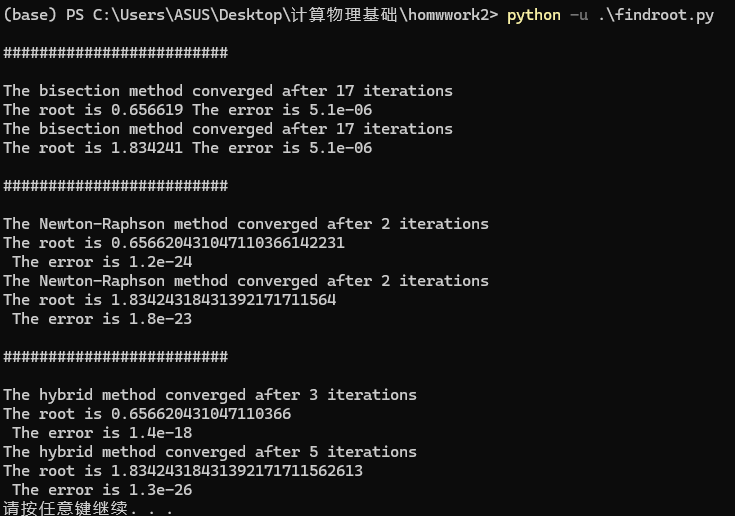
\includegraphics[width=0.6\linewidth]{photo/fig2.png}
    \caption{题目1 运行结果}
    \label{fig:2}
\end{figure}


\section{题目 2:求函数极小值}
\subsection{题目描述}
Search for the minimum of the function $g(x,y)=sin(x+y)+cos(x+2y)$ in the whole space.
\subsection{程序描述}
在本程序中,我们使用梯度下降方法来搜索g(x,y)的极小值点,其在函数$gradiant\_descent$中实现,并且,为了防止在某些位置梯度消失而导致停留在函数的鞍点上,每次下降会加上一个小的高斯噪声。

由于$sin(x)$和$cos(x)$的周期性,$g(x,y)$实际上有无数多个极值点,只需满足$x_1+y_1=2 m \pi,x_2+2y_2=2 n\pi,(m,n) \in \mathbb{Z}$。并且,由于:
$$
\begin{pmatrix}
  x \\
  y
  \end{pmatrix}=\begin{pmatrix}
    2,-1 \\
    -1,1
    
    \end{pmatrix}\begin{pmatrix}
      x+y \\
      x+2y
      \end{pmatrix}
$$
故只需要在图\ref{fig:3}(a)红线所围成的元胞中找到一个极小值点$x_0,y_0$即可,其余极小值点由$x_m=x_0+2 m\pi,y_n=y_0+2 n \pi,(m,n) \in \mathbb{Z}$给出。

本程序源文件为findmin.py,在终端进入当前目录,使用命令python -u findmin.py运行本程序。运行时请保证Python第三方库Numpy,Matplotlib已安装。程序开发环境为Python3.12.3,可在Python3.8以上版本中运行。

\subsection{伪代码}
\subsubsection*{梯度下降法伪代码:}
\begin{breakablealgorithm}
  \caption{GradiantDescent}
  \begin{algorithmic}
    \Function{GradiantDescent}{$X0,g,dg,ap,tol,maxIter$}
      \State \textbf{INPUT:} $X0$ (initial guess), $g$ (function), $dg$ (gradient of $g$), $ap$ (learning rate), $tol$ (tolerance), $maxIter$ (maximum iterations)
      \State \textbf{OUTPUT:} $X$ (final point), $his$ (history of points)
      \State $X \gets$ array($X0$) \Comment{Initialize $X$ with $X0$ as a float array}
      \State $his \gets []$ \Comment{Initialize empty history list}
      
      \For{$i \gets 1$ \To $maxIter$}
        \State $dX \gets$ $\nabla dg(X)$ \Comment{Calculate the gradient at current $X$}
        \State $X \gets X - ap \times dX + $ randomNormal($0$, $tol$) \Comment{Update $X$ with learning rate and noise}
        \State $his \gets$ append($his$, copy($X$)) \Comment{Store the current $X$ in history}
        
        \If{$||dX||$) $<$ $tol$}
          \State \textbf{Break}
        \EndIf
      \EndFor
  
    
      \State \Return $X$, $his$
    \EndFunction
  \end{algorithmic}
  \end{breakablealgorithm}
  \subsection{输入输出实例}
  对于本程序,运行后会生成图\ref{fig:3}为"find g(x,y) min.png"于当前目录下,并输出使用梯度下降法找到的极小值点。图\ref{fig:4}为程序运行截图,得到极小值为-2.00000,极小值点为
  $$Xmin=0.00000+2 m \pi,Y_min=-1.57079+2 n \pi,(m,n)\in \mathbb{Z}$$
  \begin{figure}[ht]
    \centering
    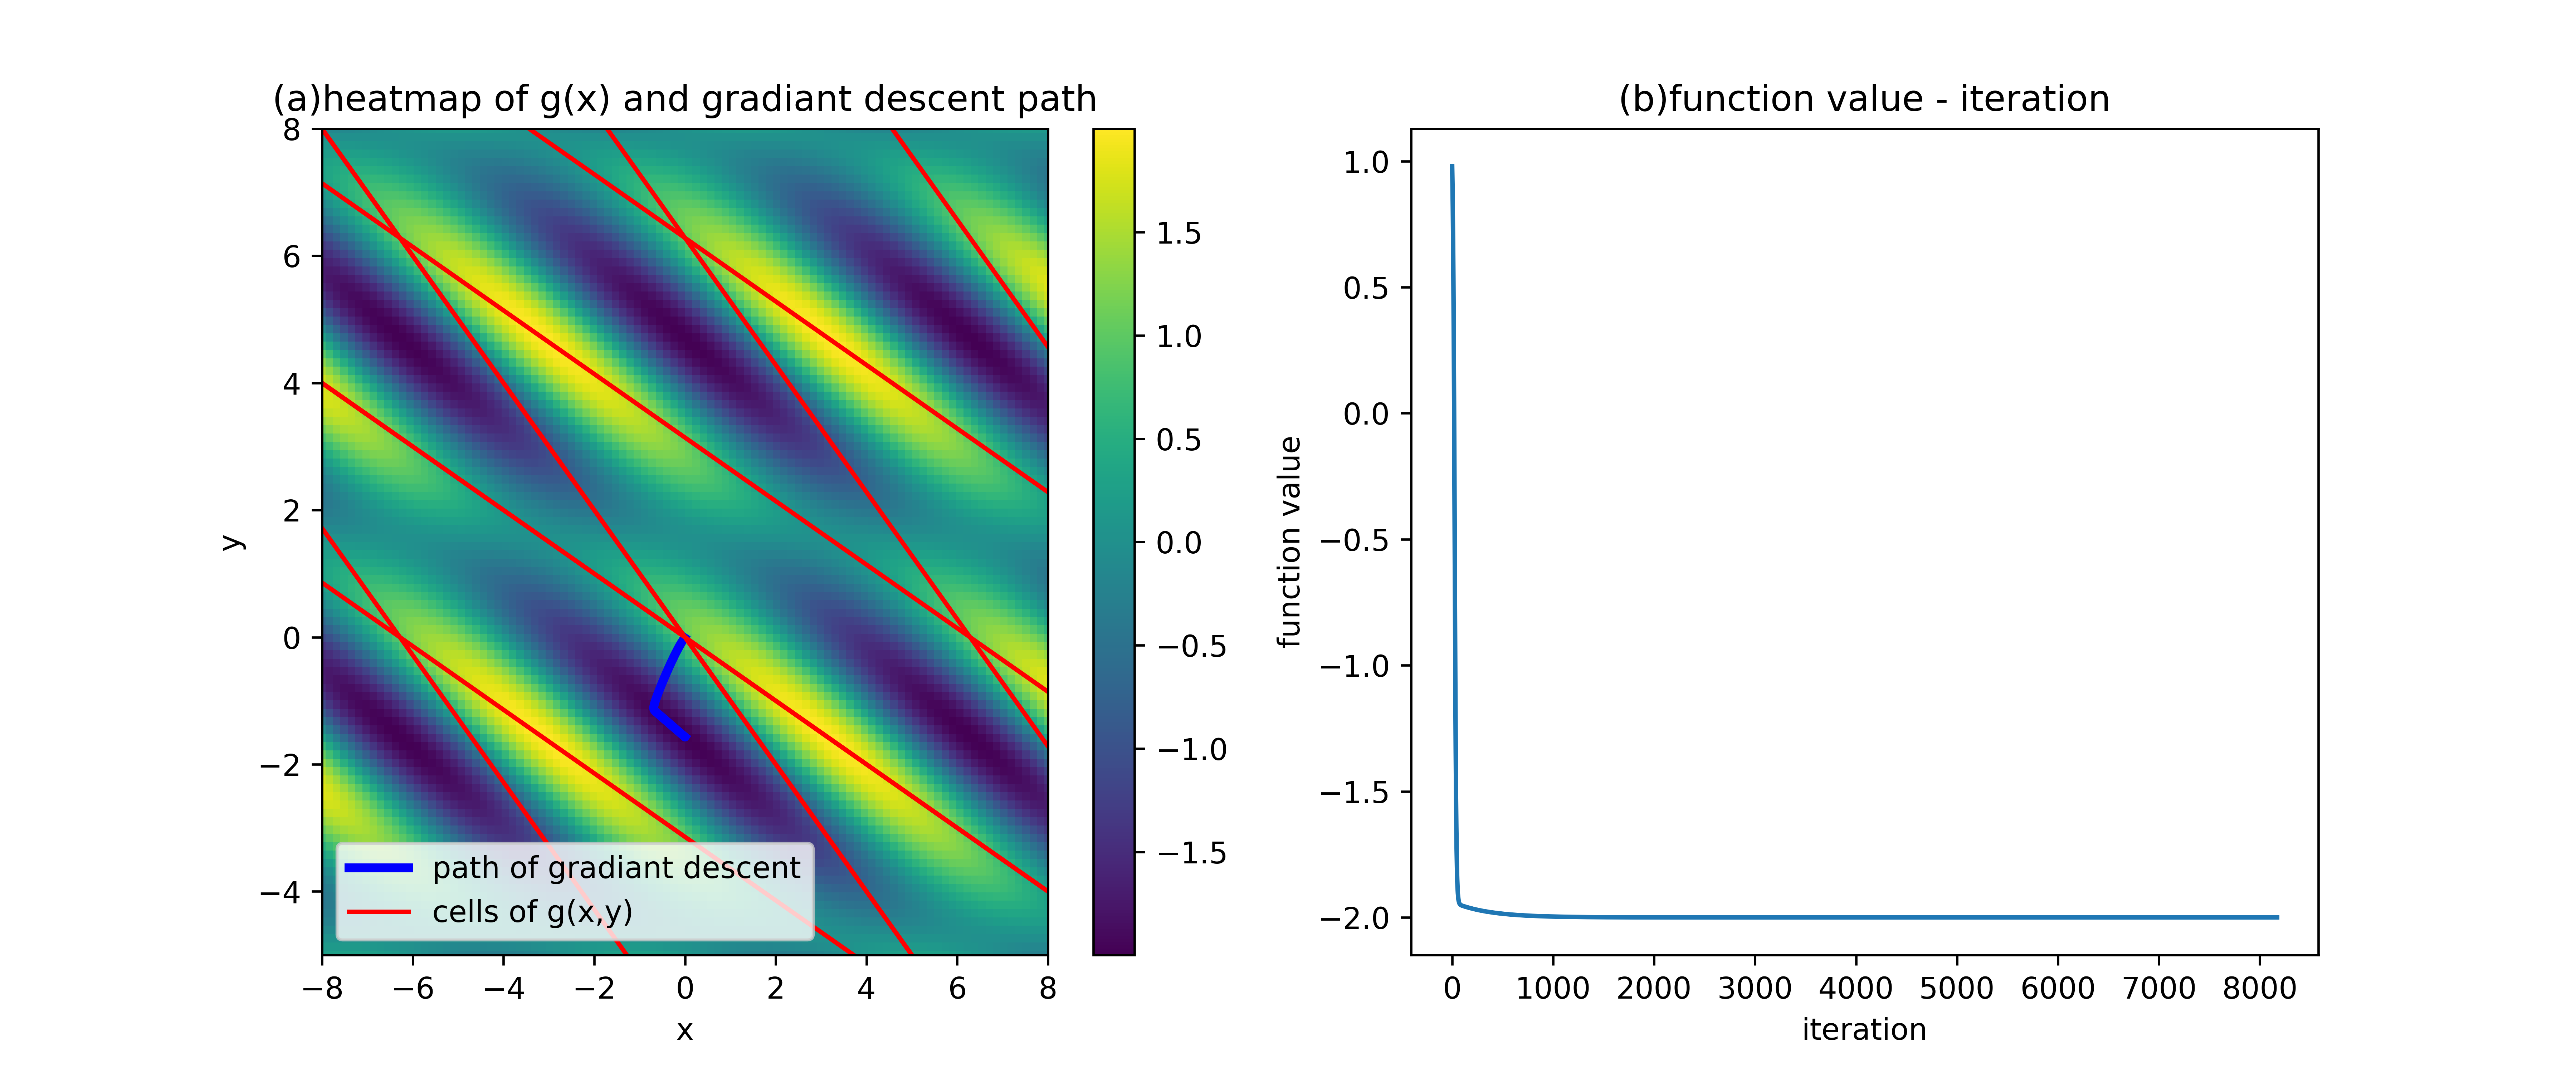
\includegraphics[width=1\linewidth]{photo/find g(x,y) min.png}
    \caption{题目2 (a)g(x,y)的热力图,用红线标注了其单元,蓝线为梯度下降路径。(b)函数值随迭代次数的变化}
    \label{fig:3}
  \end{figure}
  \begin{figure}[ht]
    \centering
    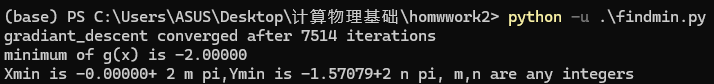
\includegraphics[width=0.6\linewidth]{photo/fig4.png}
    \caption{题目2程序运行截图}
    \label{fig:4}
  \end{figure}

  \section{题目3}
  \subsection{题目描述}
  Electron in the finite square-well potential is,  $(V_0=10eV,a=0.2 nm)$
  $$
  V(x)=\begin{cases} 
    V_0, & \text{if } x \leq -a ,\textbf{Region \uppercase\expandafter{\romannumeral 1}}\\
    0, & \text{if } -a< x < a ,\textbf{Region \uppercase\expandafter{\romannumeral 2}}\\ V_0, & \text{if } x \geq a ,\textbf{Region \uppercase\expandafter{\romannumeral 3}}\\
 \end{cases}
  $$
Find the three lowest eigen states (both energies and wavefunctions).
  \begin{figure}[ht]
    \centering
    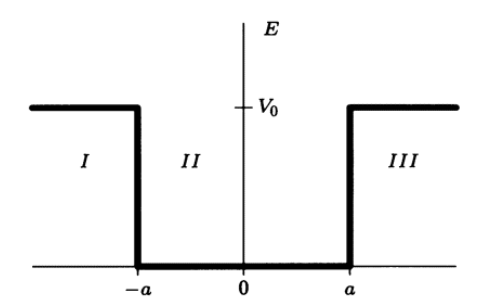
\includegraphics[width=0.6\linewidth]{photo/fig5.png}
    \caption{题目3方势阱示意图}
    \label{fig:5}
  \end{figure}
\subsection{程序描述}
在本程序中,我们通过求解奇、偶宇称的波函数的边界条件方程:$f_{odd}=\alpha sin \alpha a+\beta cos \alpha a=0$和$f_{even}=\alpha sin\alpha a+\beta cos\alpha=0$,其中$\alpha =\sqrt{2 m E}/\hbar^2,\beta=\sqrt{2 m(V_0-E)}/\hbar$,得到波函数的三个能量最小的束缚态(由图\ref{fig:6}可看出事实上只存在3个束缚态)。

对$f_{even}$和$f_{odd}$的求根使用在题目1中实现的$bisection\_method$实现,并重新计算出A,B,C,D系数得到波函数。接着对波函数的平方进行积分,将波函数归一化。积分在$int_Trapezoidal$中使用梯形法实现,即$N_e=h(1/2 \rho_0+rho_1+...+\rho_{N-1}+1/2\rho_N)$,其中$h={b-a\over N},a,b$为上下界,$N$为采样点数。由于$|x|>a$波函数为指数下降,因此我们对波函数在$|x|>10a$处截断。

为了降低数值误差,本程序中能量单位采用$eV$,长度单位采用$nm$,并定义常数$k={2 m_e\over\hbar^2}=26.24684351 nm^{-1}\cdot eV^{-1}$

本程序源文件为solvesqurepotential.py,在终端进入当前目录,使用命令python -u solvesqurepotential.py运行本程序。运行时请保证此程序与题目1程序findroot.py在同一文件夹下,且Python第三方库Numpy,Matplotlib已安装。程序开发环境为Python3.12.3,可在Python3.8以上版本中运行。

\subsection{伪代码}
\subsubsection{Trapezoidal integrate 伪代码:}
\begin{breakablealgorithm}
  \caption{IntTrapezoidal}
  \begin{algorithmic}
    \Function{IntTrapezoidal}{$f, a, b, n$}
      \State \textbf{INPUT:} $f$ (function), $a$ (lower limit), $b$ (upper limit), $n$ (number of points)
      \State \textbf{OUTPUT:} $intfx$ (integration result)
  
      \State $x \gets \text{linspace}(a, b, n+1)$ \Comment{Generate $n+1$ points between $a$ and $b$}
      \State $intfx \gets \left(\sum_{i=0}^{n}f(x[i]) - \frac{1}{2}f(x[0]) - \frac{1}{2}f(x[n])\right) \cdot \frac{b - a}{n}$
      
      \State \Return $intfx$
    \EndFunction
  \end{algorithmic}
  \end{breakablealgorithm}
  
  \begin{breakablealgorithm}
  \caption{Calculate the wave function}
  \begin{algorithmic}
    \State $Ei, erri \gets$ BisectionMethod($fEven/odd, bracketEven/odd[0]$)
    \State $F \gets 1$
    \If{Even Wave Fucntion}
      \State $A\gets 0$ ,$C\gets F$ ,$B \gets Fe^{-\beta a}/cos({\alpha a})$
    \ElsIf{Odd Wave Function}
      \State $B \gets F$ ,$C\gets -F$
      \State $A \gets Fe^{-\beta a}/sin({\alpha a})$
      \Comment{Calculate A,B,C,F}
    \EndIf
    \State $norm \gets$ IntTrapezoidal($f, -10a, 10a, 1000$)
    $A,B,C,F \gets (A,B,C,F)/norm$
    \Comment{Normalize the wave function}
    \State{Plot and Output the wave function}
  \end{algorithmic}
  \end{breakablealgorithm}
  \begin{figure}[ht]
    \centering
    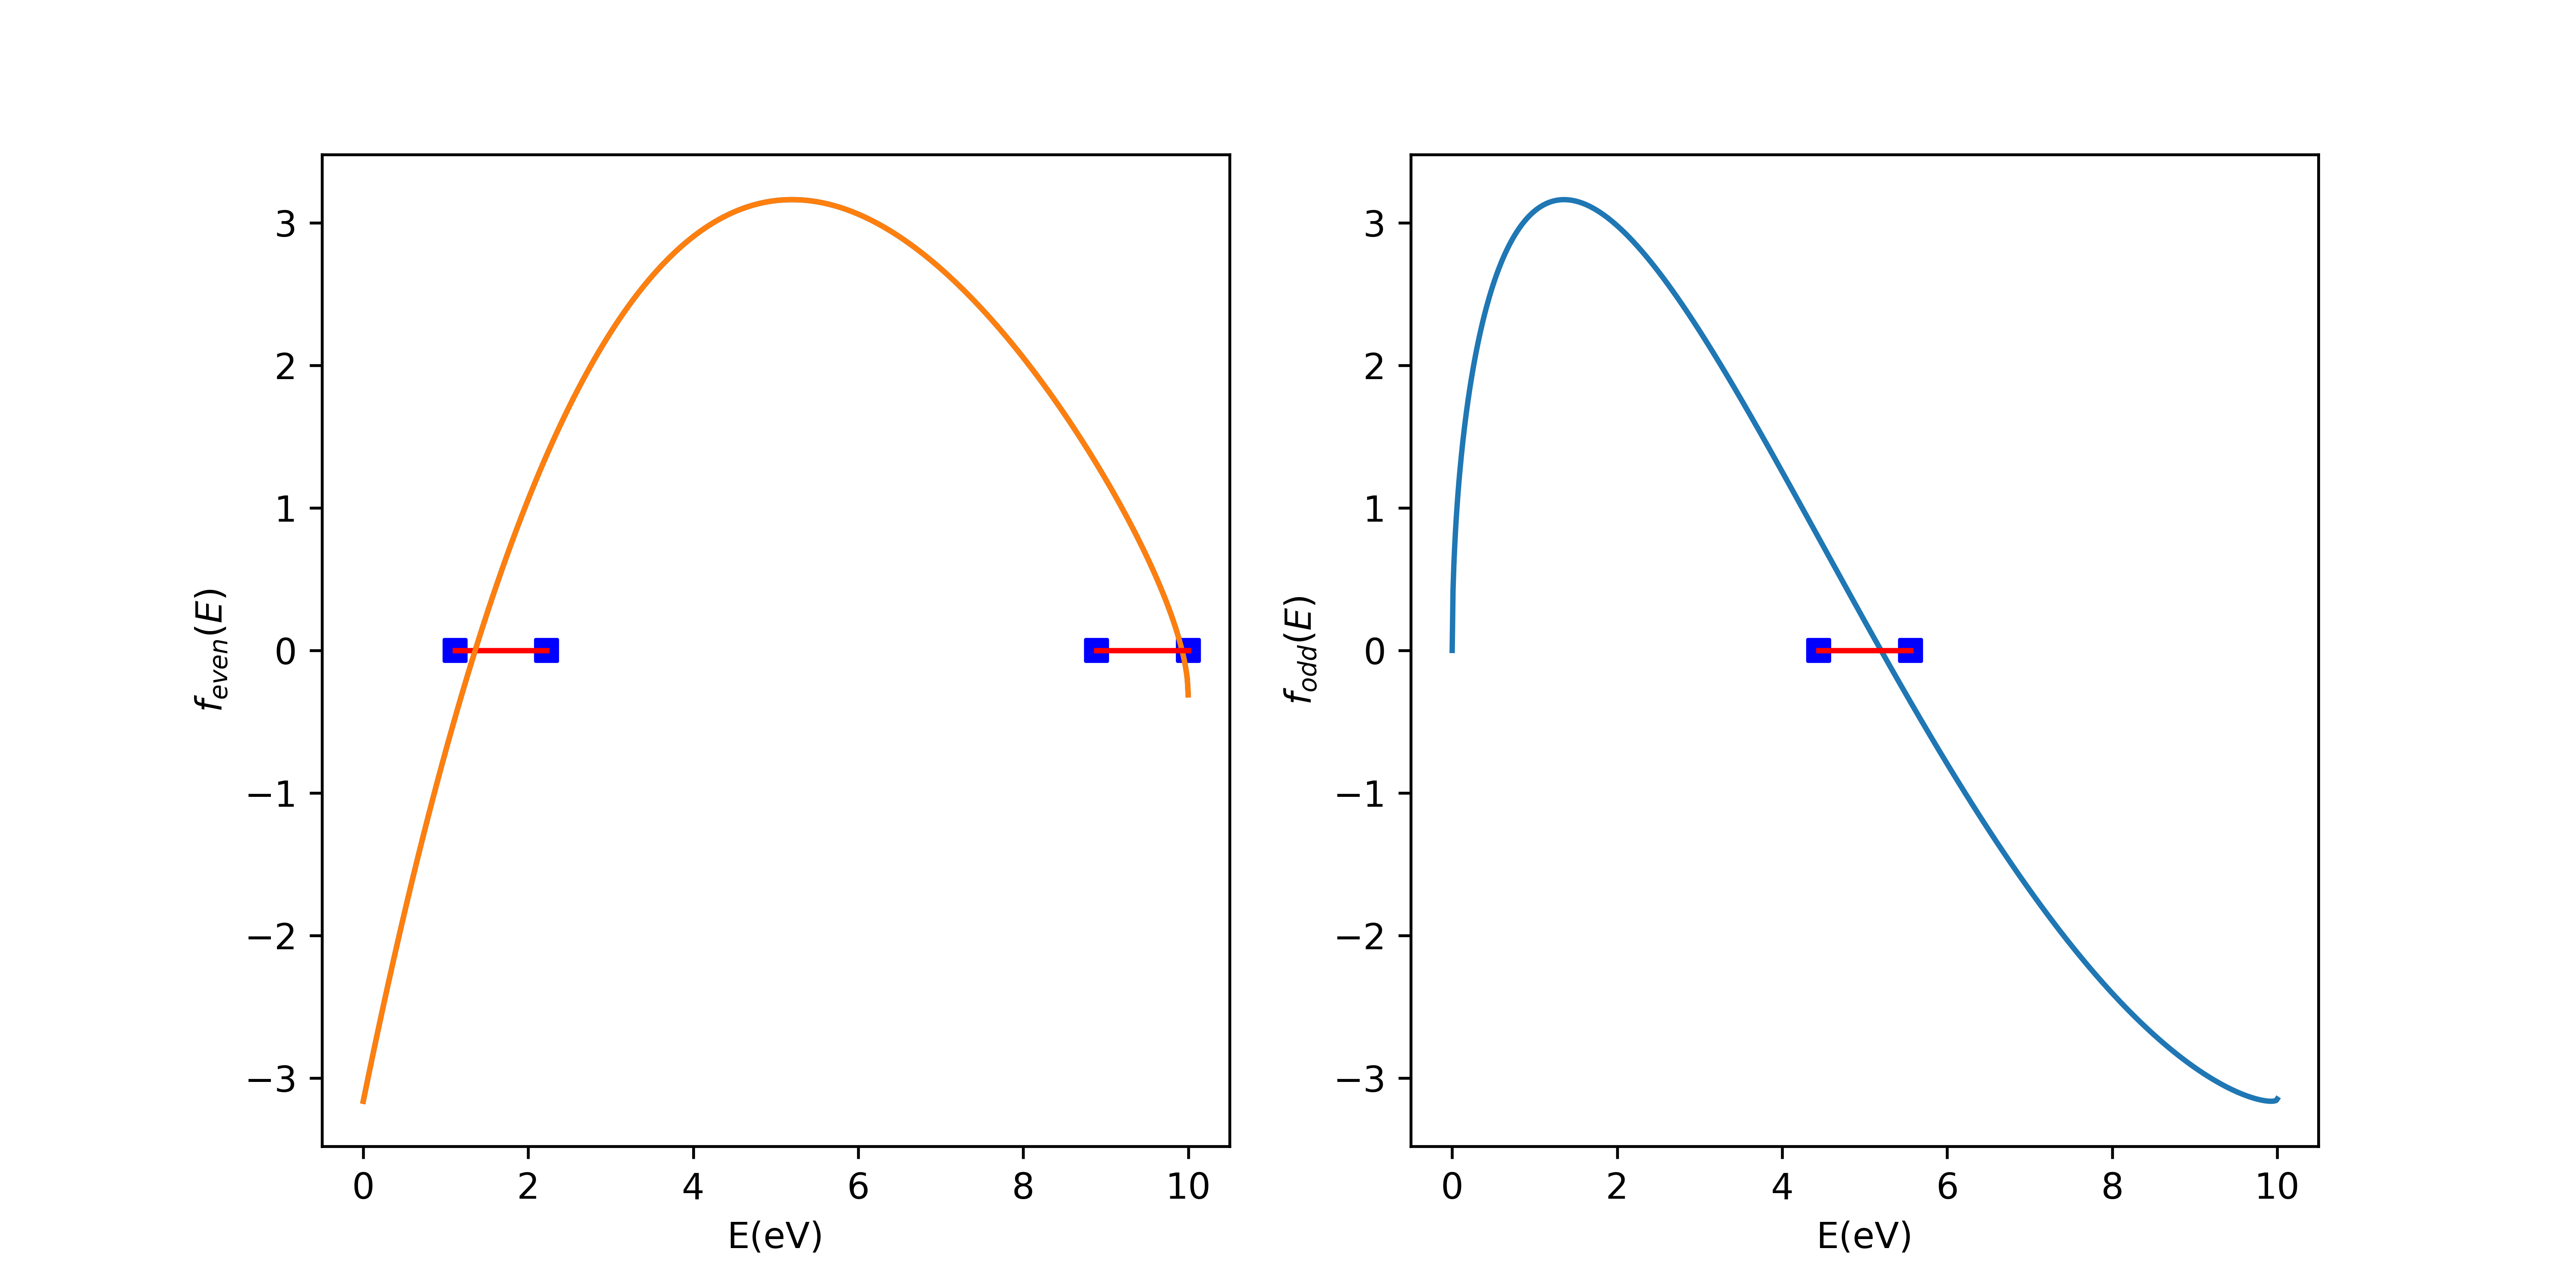
\includegraphics[width=0.8\linewidth]{photo/f_even and f_odd.png}
    \caption{$f_{odd}$和$f_{even}$根位置示意图}
    \label{fig:6}
  \end{figure}
  \subsection{输入输出实例}
  对于本程序,运行后会生成图\ref{fig:6}为"f\_even and f\_odd.png"和\ref{fig:7}为"wavefunction.png"于当前目录下,并输出三个束缚态的能量和波函数表达式。图\ref{fig:8}为程序运行截图。程序得到束缚态能量为$E_0=1.35689 eV,E_1=5.19897 eV,E_2=9.92541 eV$,波函数表达式分别为($x$单位为$nm$)
   

$$
\psi_0(x) = 
\begin{cases} 
14.51282 \, e^{-15.06168 \, x}, & x > a \\
14.51282 \, e^{15.06168 \, x}, & x < -a \\
1.93748 \, \cos(5.96776 \, x), & -a \leq x \leq a
\end{cases}
$$
  

  $$
  \psi_1(x) = 
  \begin{cases} 
  12.66141 \, e^{-11.22550 \, x}, & x > a \\
  -12.66141 \, e^{11.22550 \, x}, & x < -a \\
  1.85990 \, \sin(11.68146 \, x), & -a \leq x \leq a
  \end{cases}
  $$
  

  $$
  \psi_2(x) = 
  \begin{cases} 
    1.38157 \, e^{-1.39923 \, x}, & x > a \\
    1.38157 \, e^{1.39923 \, x}, & x < -a \\
  -1.04824 \, \cos(16.14034 \, x), & -a \leq x \leq a
  \end{cases}
  $$
  
  \begin{figure}[ht]
    \centering
    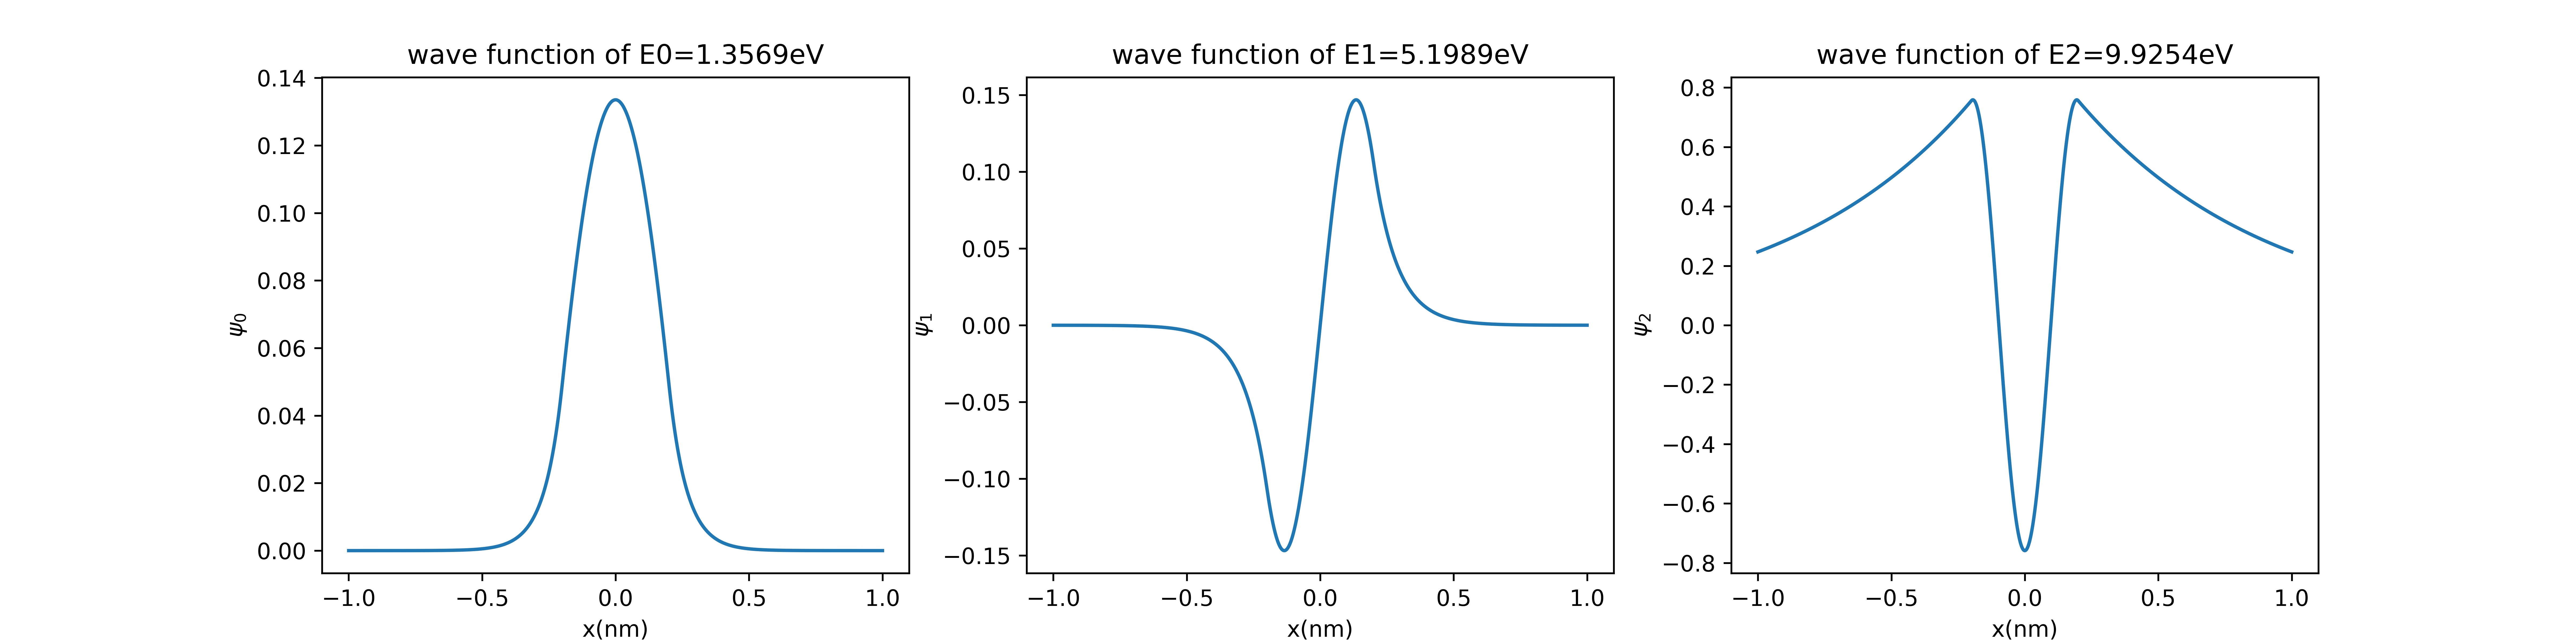
\includegraphics[width=1\linewidth]{photo/wavefunction.png}
    \caption{不同能量的波函数图像}
    \label{fig:7}
  \end{figure}
  \begin{figure}[ht]
    \centering
    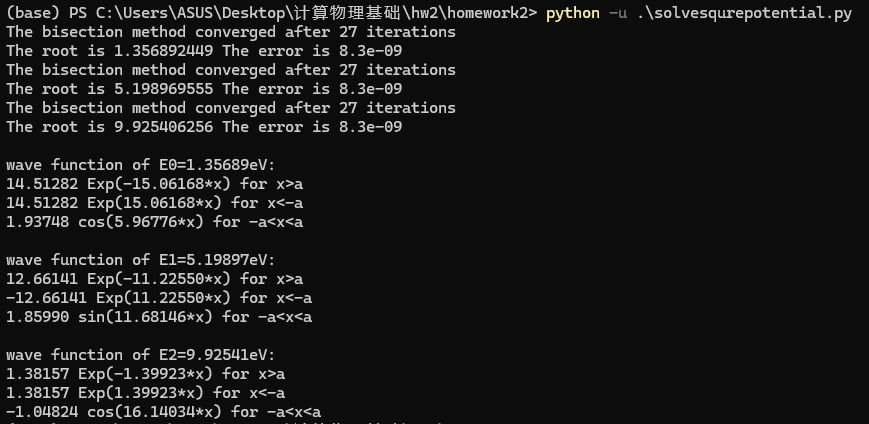
\includegraphics[width=0.8\linewidth]{photo/fig8.png}
    \caption{题目3程序运行截图}
    \label{fig:8}
  \end{figure}
\end{document}


